\documentclass{article}
\usepackage[UTF8]{ctex}
\usepackage{geometry}
\usepackage{makecell}
\usepackage{amsmath}
\usepackage{graphicx}
\usepackage{bigstrut}
\usepackage{subfigure}
\usepackage{float}

\geometry{a4paper,scale=0.75}

\title{\heiti 实验二十五\ 动态法测良导体热导率}
\author{\kaishu 田睿轩\ 物理学院\ 1900011602}
\date{2021年5月6日}
\newcommand{\degree}{^\circ}
\newcommand{\degreesCelsius}{^\circ C}

\begin{document}
    \maketitle
    \section{实验数据及处理}
    实验所用良导体中的热传导可视为一维热传导,满足方程
    $$\frac{\partial T}{\partial t}=\alpha \frac{\partial^{2} T}{\partial x^{2}}$$
    其中$\alpha=\frac{\kappa}{c\rho}$为热扩散率。

    实验中,通过在冷端使用冷却水使冷端温度保持为$T_0$,热端通过加热器和冷却水交替加热冷却,使其温度简谐变化,满足:
    $$T=T_{0}+T_{\mathrm{m}} \sin \omega t$$

    于是,棒中的温度分布满足:
    $$T=T_{0}-k x+T_{\mathrm{m}} \mathrm{e}^{-\sqrt{\frac{s}{2} x} x} \sin \left(\omega t-\sqrt{\frac{\omega}{2 \alpha}} x\right)$$

    由此可见,棒中的温度分布为衰减波。而对于某一特定位置处,温度随时间的变化曲线应为正(余)线曲线。实验中,通过八个等间隔分布的热电偶
    测量不同位置处的温度随时间的变化情况并绘制成八条曲线,通过热波的峰或谷传到不同位置的时间差可以计算出热波波速进而计算出热导率。
    实验中,由于热端的温度无法完全按照简谐变化,因此实际上的热波也不是完全的正弦波,但由于高次谐波衰减快,因此可近似看为正弦波。
    实验中调节热端的冷却水的流量,使得测得的曲线尽可能的对称,接近于正弦波。调节完冷却水流量并待温度稳定后,选取五个连续的峰谷进行计算。

    曲线稳定后测得冷端水量为$400ml/min$,热端水量为$900ml/min$。选取的五簇连续的曲线簇中,峰峰值分别如表1所示,相对误差小于$2\%$,可以认为基本达到稳定,满足实验所需条件。
    \begin{table}[h]
        \centering
        \caption{选取曲线簇峰峰值}
        \vspace{1ex}
        \begin{tabular}{ccccccccc}
            \hline
                  & 1     & 2     & 3     & 4     & 5     & 平均    & 最大-最小 & (最大-最小)/平均 \bigstrut[t]\\
            峰峰值/mV & 175.4 & 174.8 & 174.3 & 174.9 & 177.7 & 175.4  & 3.4   & 1.9\% \bigstrut[b]\\
            \hline
        \end{tabular}%
    \end{table}

    实验中取一簇峰和两簇谷,然后计算每个峰与第一个峰之间的时间差$t_{i+1}-t_{1}(i=1,2,...,7)$,由于热波的波速满足$v=i l_{0} /\left(t_{i+1}-t_{1}\right)$,所以
    每个峰与第一个峰之间的时间差满足$t_{i+1}-t_{1}=\frac{i l_{0}}{v}$,因此,用最小二乘法拟合$\left(t_{i+1}-t_{1}\right)-i$曲线,即可用斜率计算出波速进而求出热导率。

    \subsection{峰曲线簇}
    取一个峰曲线簇,记录不同位置的达峰时间,如表2所示。
    \begin{table}[h]
        \centering
        \caption{峰曲线簇各位置达峰时间}
        \vspace{1ex}
        \begin{tabular}{ccccccccc}
            \hline
                  & 1     & 2     & 3     & 4     & 5     & 6     & 7     & 8 \bigstrut[t]\\
            $t_{\text{峰}1}/s$ & 4602.95 & 4609.60 & 4617.57 & 4625.55 & 4629.54 & 4640.17 & 4649.48 & 4657.46 \\
            $V_{\text{峰}1}/mV$ & 755.5 & 654.5 & 576.0   & 508.8 & 452.8 & 501.5 & 354.0   & 312.6 \bigstrut[b]\\
            \hline
        \end{tabular}%
    \end{table}

    对曲线簇的达峰时间差用最小二乘法绘制$\left(t_{i+1}-t_{1}\right)-i$曲线,如图1所示:

    \begin{figure*}[h]
        \centering
        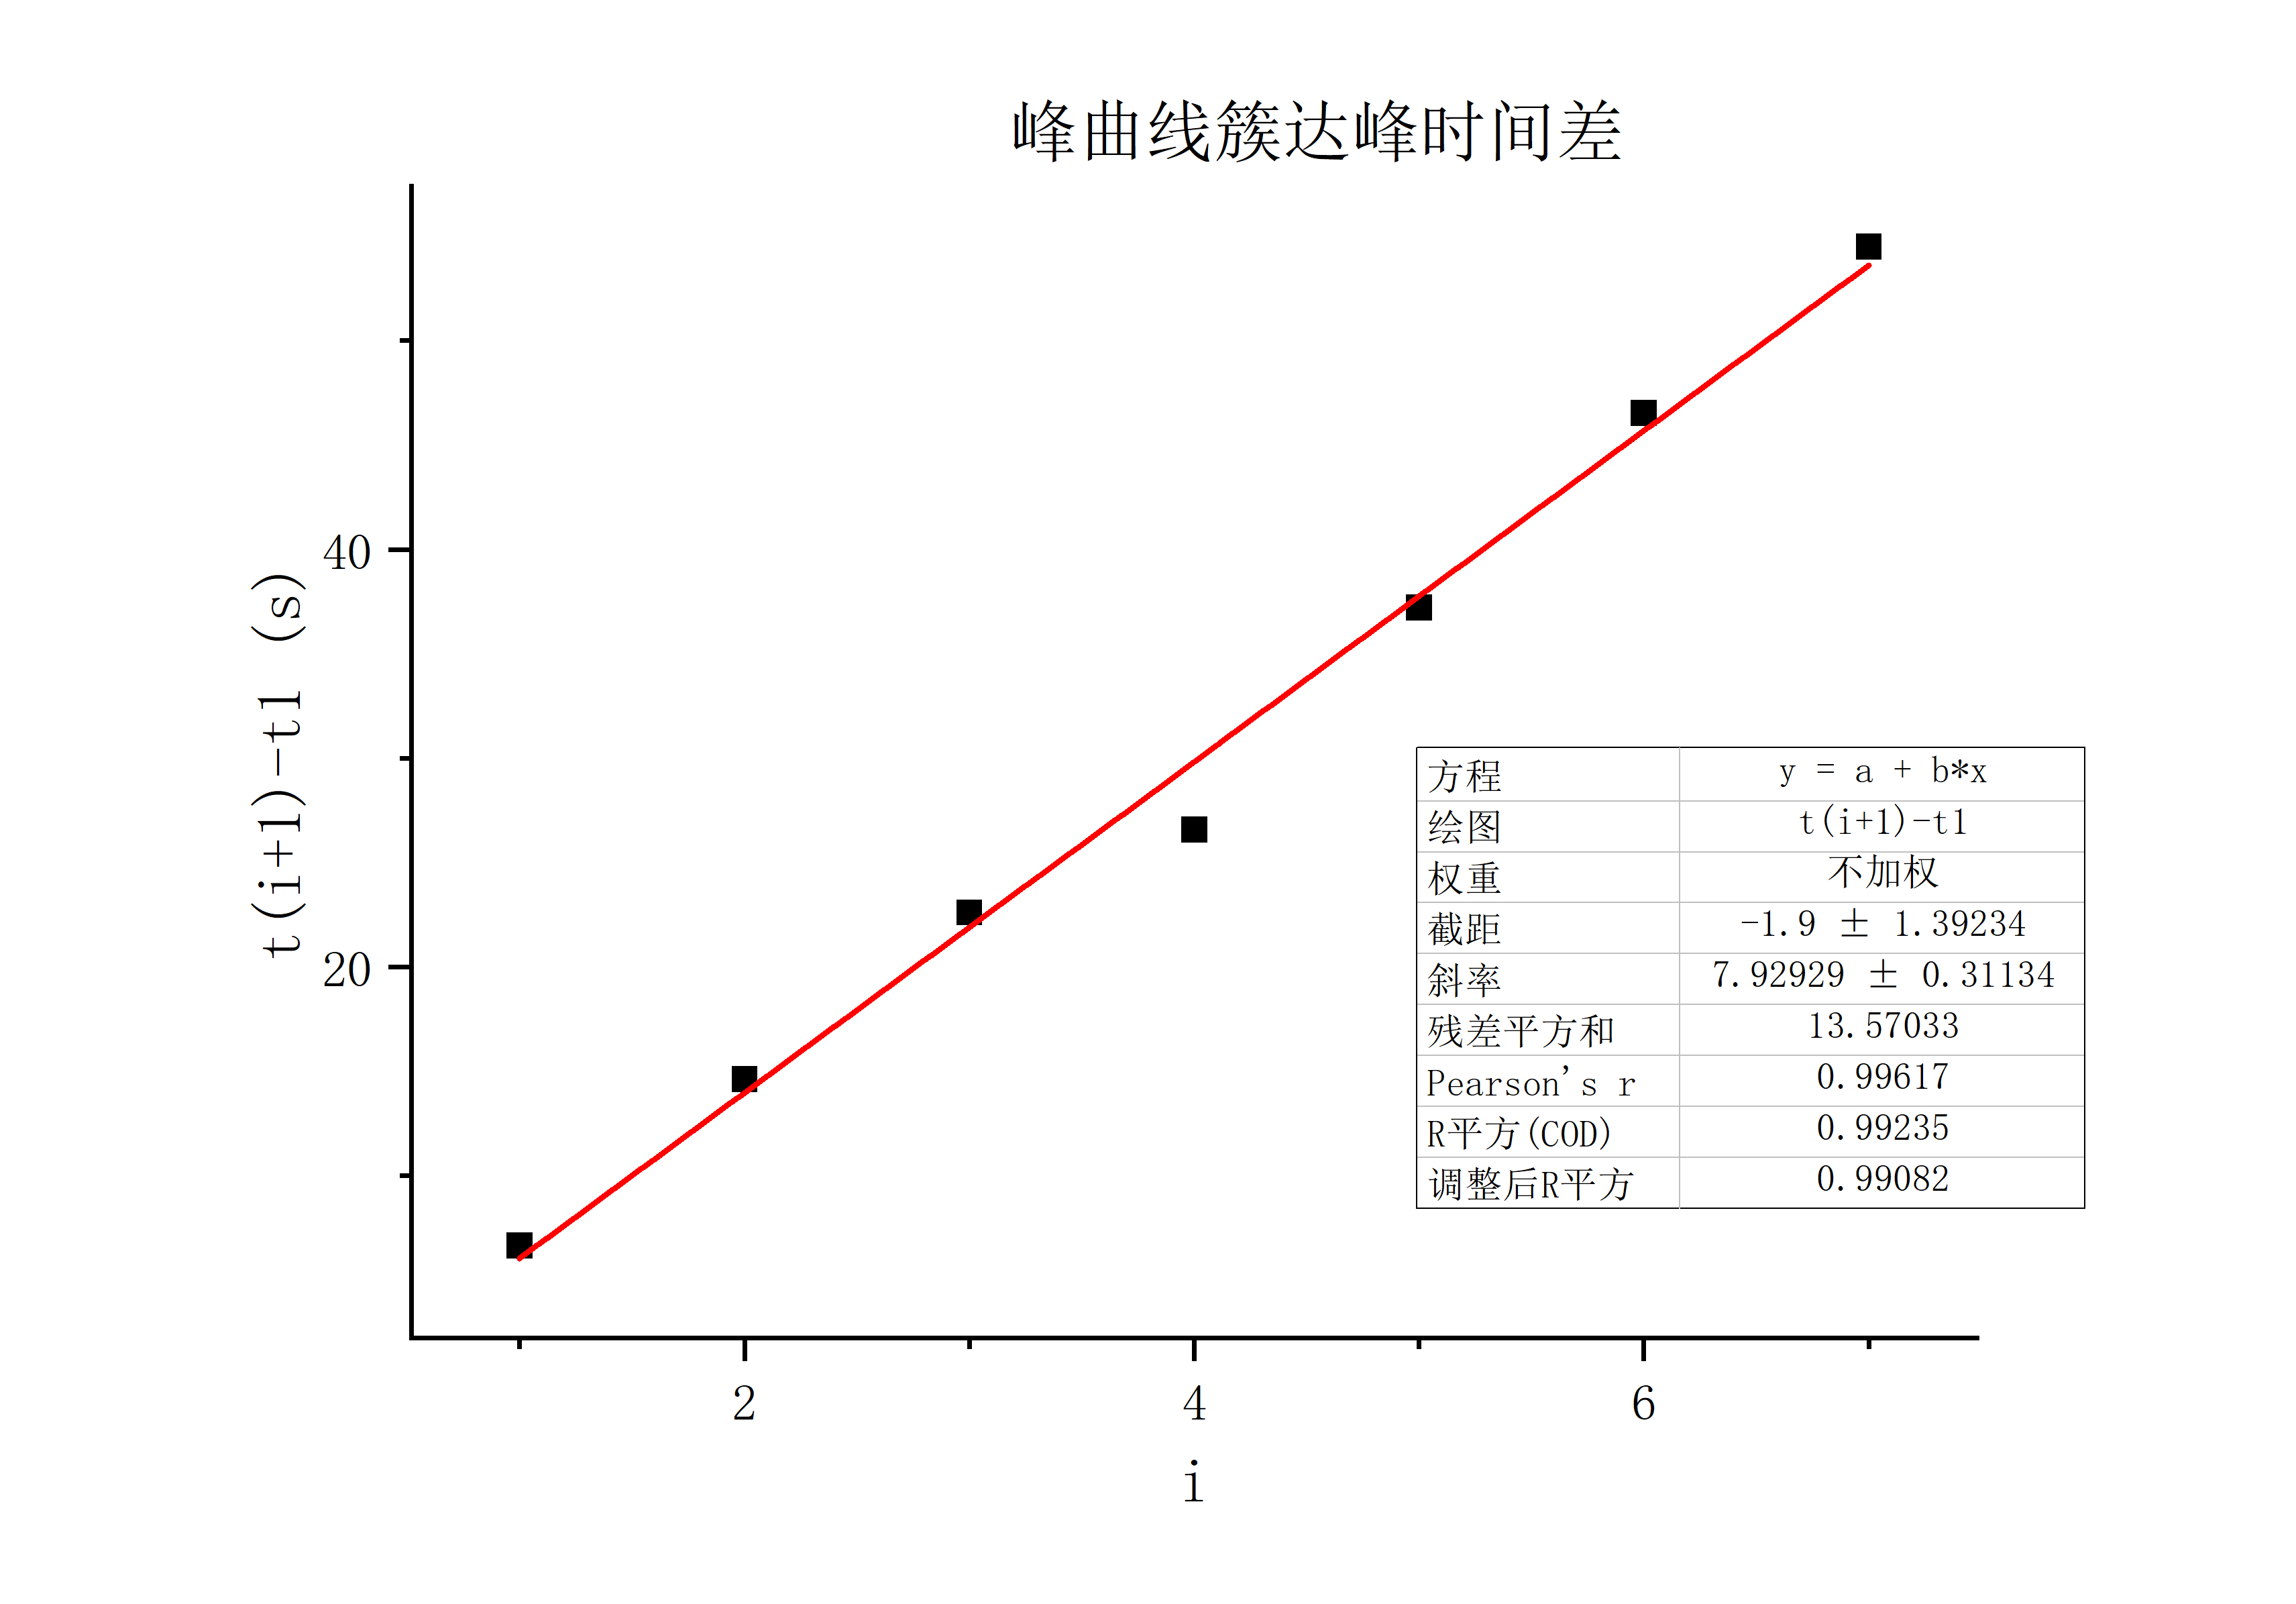
\includegraphics[width=0.7\textwidth]{峰.jpg}
        \caption{峰曲线簇达峰时间差}
    \end{figure*}

    曲线斜率$k=7.93s$,相关系数$r=0.996$。由此可计算得热波波速$v=\frac{l_0}{k}=2.52\times 10^{-3}m/s$。取铝的密度为
    $\rho_{A l}=2.70 \times 10^{3} \mathrm{~kg} \cdot \mathrm{m}^{-3}$,铝的比热为$C_{A l}=0.89 \times 10^{3} \mathrm{~J} \cdot \mathrm{kg}^{-1} \cdot \mathrm{K}^{-1}$,
    热端温度变化周期为180s。于是可以计算得到热导率
    $$\kappa=\frac{v^{2} c \rho}{4 \pi f}=\frac{v^{2} c \rho}{4 \pi} T_{\text {period }}=218W/m\cdot K$$

    用实验室提供的软件可以对曲线簇在峰值附近进行正弦函数拟合,然后根据拟合后的函数寻峰并利用最小二乘法计算热波波速,使用该软件利用峰曲线簇计算得到的波速为
    $$\kappa'=233.66W/m\cdot K$$

    \subsection{谷1曲线簇}
    取一个谷曲线簇,读出其中各曲线谷所对应的时间,如表3所示。

    \begin{table}[h]
        \centering
        \caption{谷1曲线簇各位置达谷时间}
        \vspace{1ex}
        \begin{tabular}{ccccccccc}
            \hline
                  & 1     & 2     & 3     & 4     & 5     & 6     & 7     & 8 \bigstrut[t]\\
            $t_{\text{谷}1}/s$ & 4697.34  & 4705.31  & 4713.29  & 4721.27  & 4730.57  & 4735.89  & 4746.52  & 4754.50  \\
            $v_{\text{谷}1}/mV$ & 576.4  & 528.7  & 483.5  & 442.0  & 402.6  & 363.7  & 325.9  & 292.0  \bigstrut[b]\\
            \hline
        \end{tabular}%    
    \end{table}

    对谷1曲线簇达谷时间差用最小二乘法绘制$\left(t_{i+1}-t_{1} \right)-i$曲线,如图2所示。
    
    \begin{figure*}[h]
        \centering
        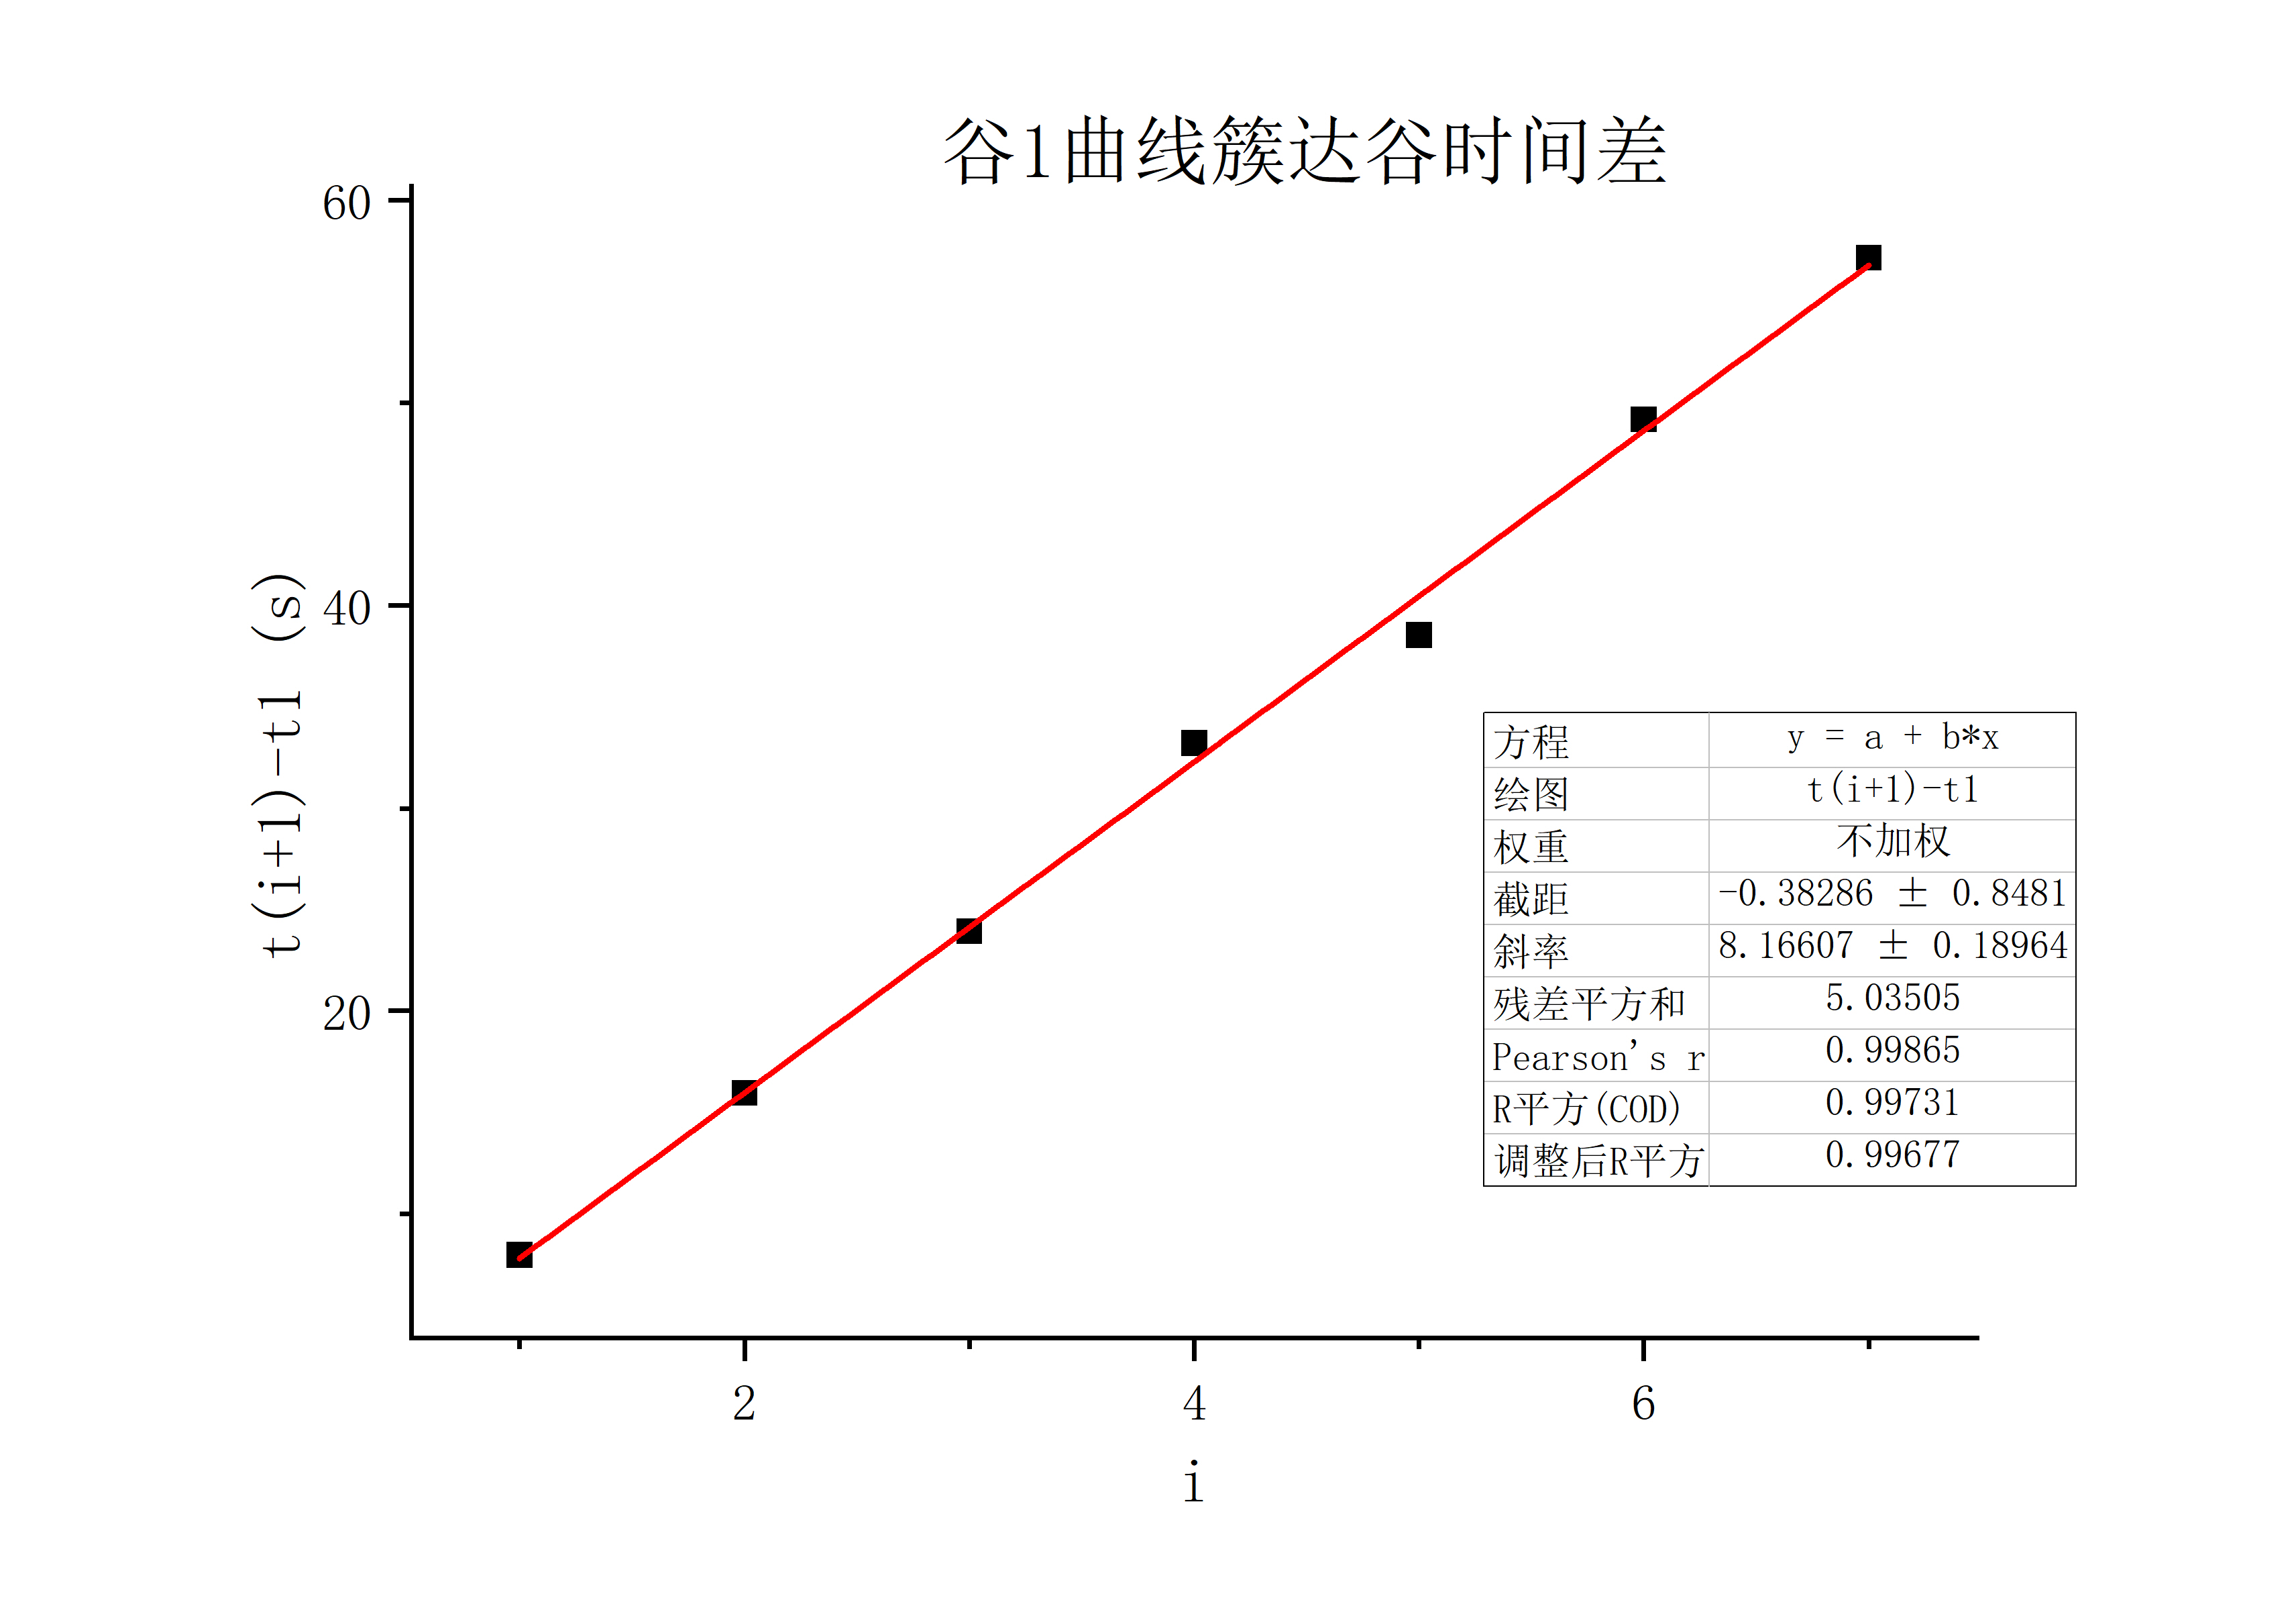
\includegraphics[width=0.7\textwidth]{谷1.jpg}
        \caption{谷1曲线簇达谷时间差}
    \end{figure*}

    曲线斜率$k=8.17s$,相关系数$r=0.999$。由此可计算得热波波速$v=\frac{l_0}{k}=2.45\times 10^{-3}m/s$。
    计算得到热导率
    $$\kappa=\frac{v^{2} c \rho}{4 \pi f}=\frac{v^{2} c \rho}{4 \pi} T_{\text {period }}=206W/m\cdot K$$

    用实验室提供的软件可以对曲线簇在峰值附近进行正弦函数拟合,然后根据拟合后的函数寻峰并利用最小二乘法计算热波波速,使用该软件利用峰曲线簇计算得到的波速为
    $$\kappa'=240.88W/m\cdot K$$

    \subsection{谷2曲线簇}
    再取另外一个谷曲线簇,读出其中各曲线谷所对应的时间,如表4所示。

    \begin{table}[h]
        \centering
        \caption{谷2曲线簇各位置达谷时间}
        \vspace{1ex}
        \begin{tabular}{ccccccccc}
            \hline
                  & 1     & 2     & 3     & 4     & 5     & 6     & 7     & 8 \bigstrut[t]\\
            $t_{\text{谷}2}/s$ & 4876.81  & 4884.78  & 4892.76  & 4900.73  & 4907.38  & 4916.69  & 4927.32  & 4933.97  \\
            $v_{\text{谷}2}/mV$ & 577.1  & 528.7  & 483.4  & 440.5  & 401.8  & 362.7  & 325.9  & 290.6  \bigstrut[b]\\
            \hline
        \end{tabular}%            
    \end{table}

    对谷2曲线簇达谷时间差用最小二乘法绘制$\left(t_{i+1}-t_{1} \right)-i$曲线,如图3所示。
    \begin{figure*}[h]
        \centering
        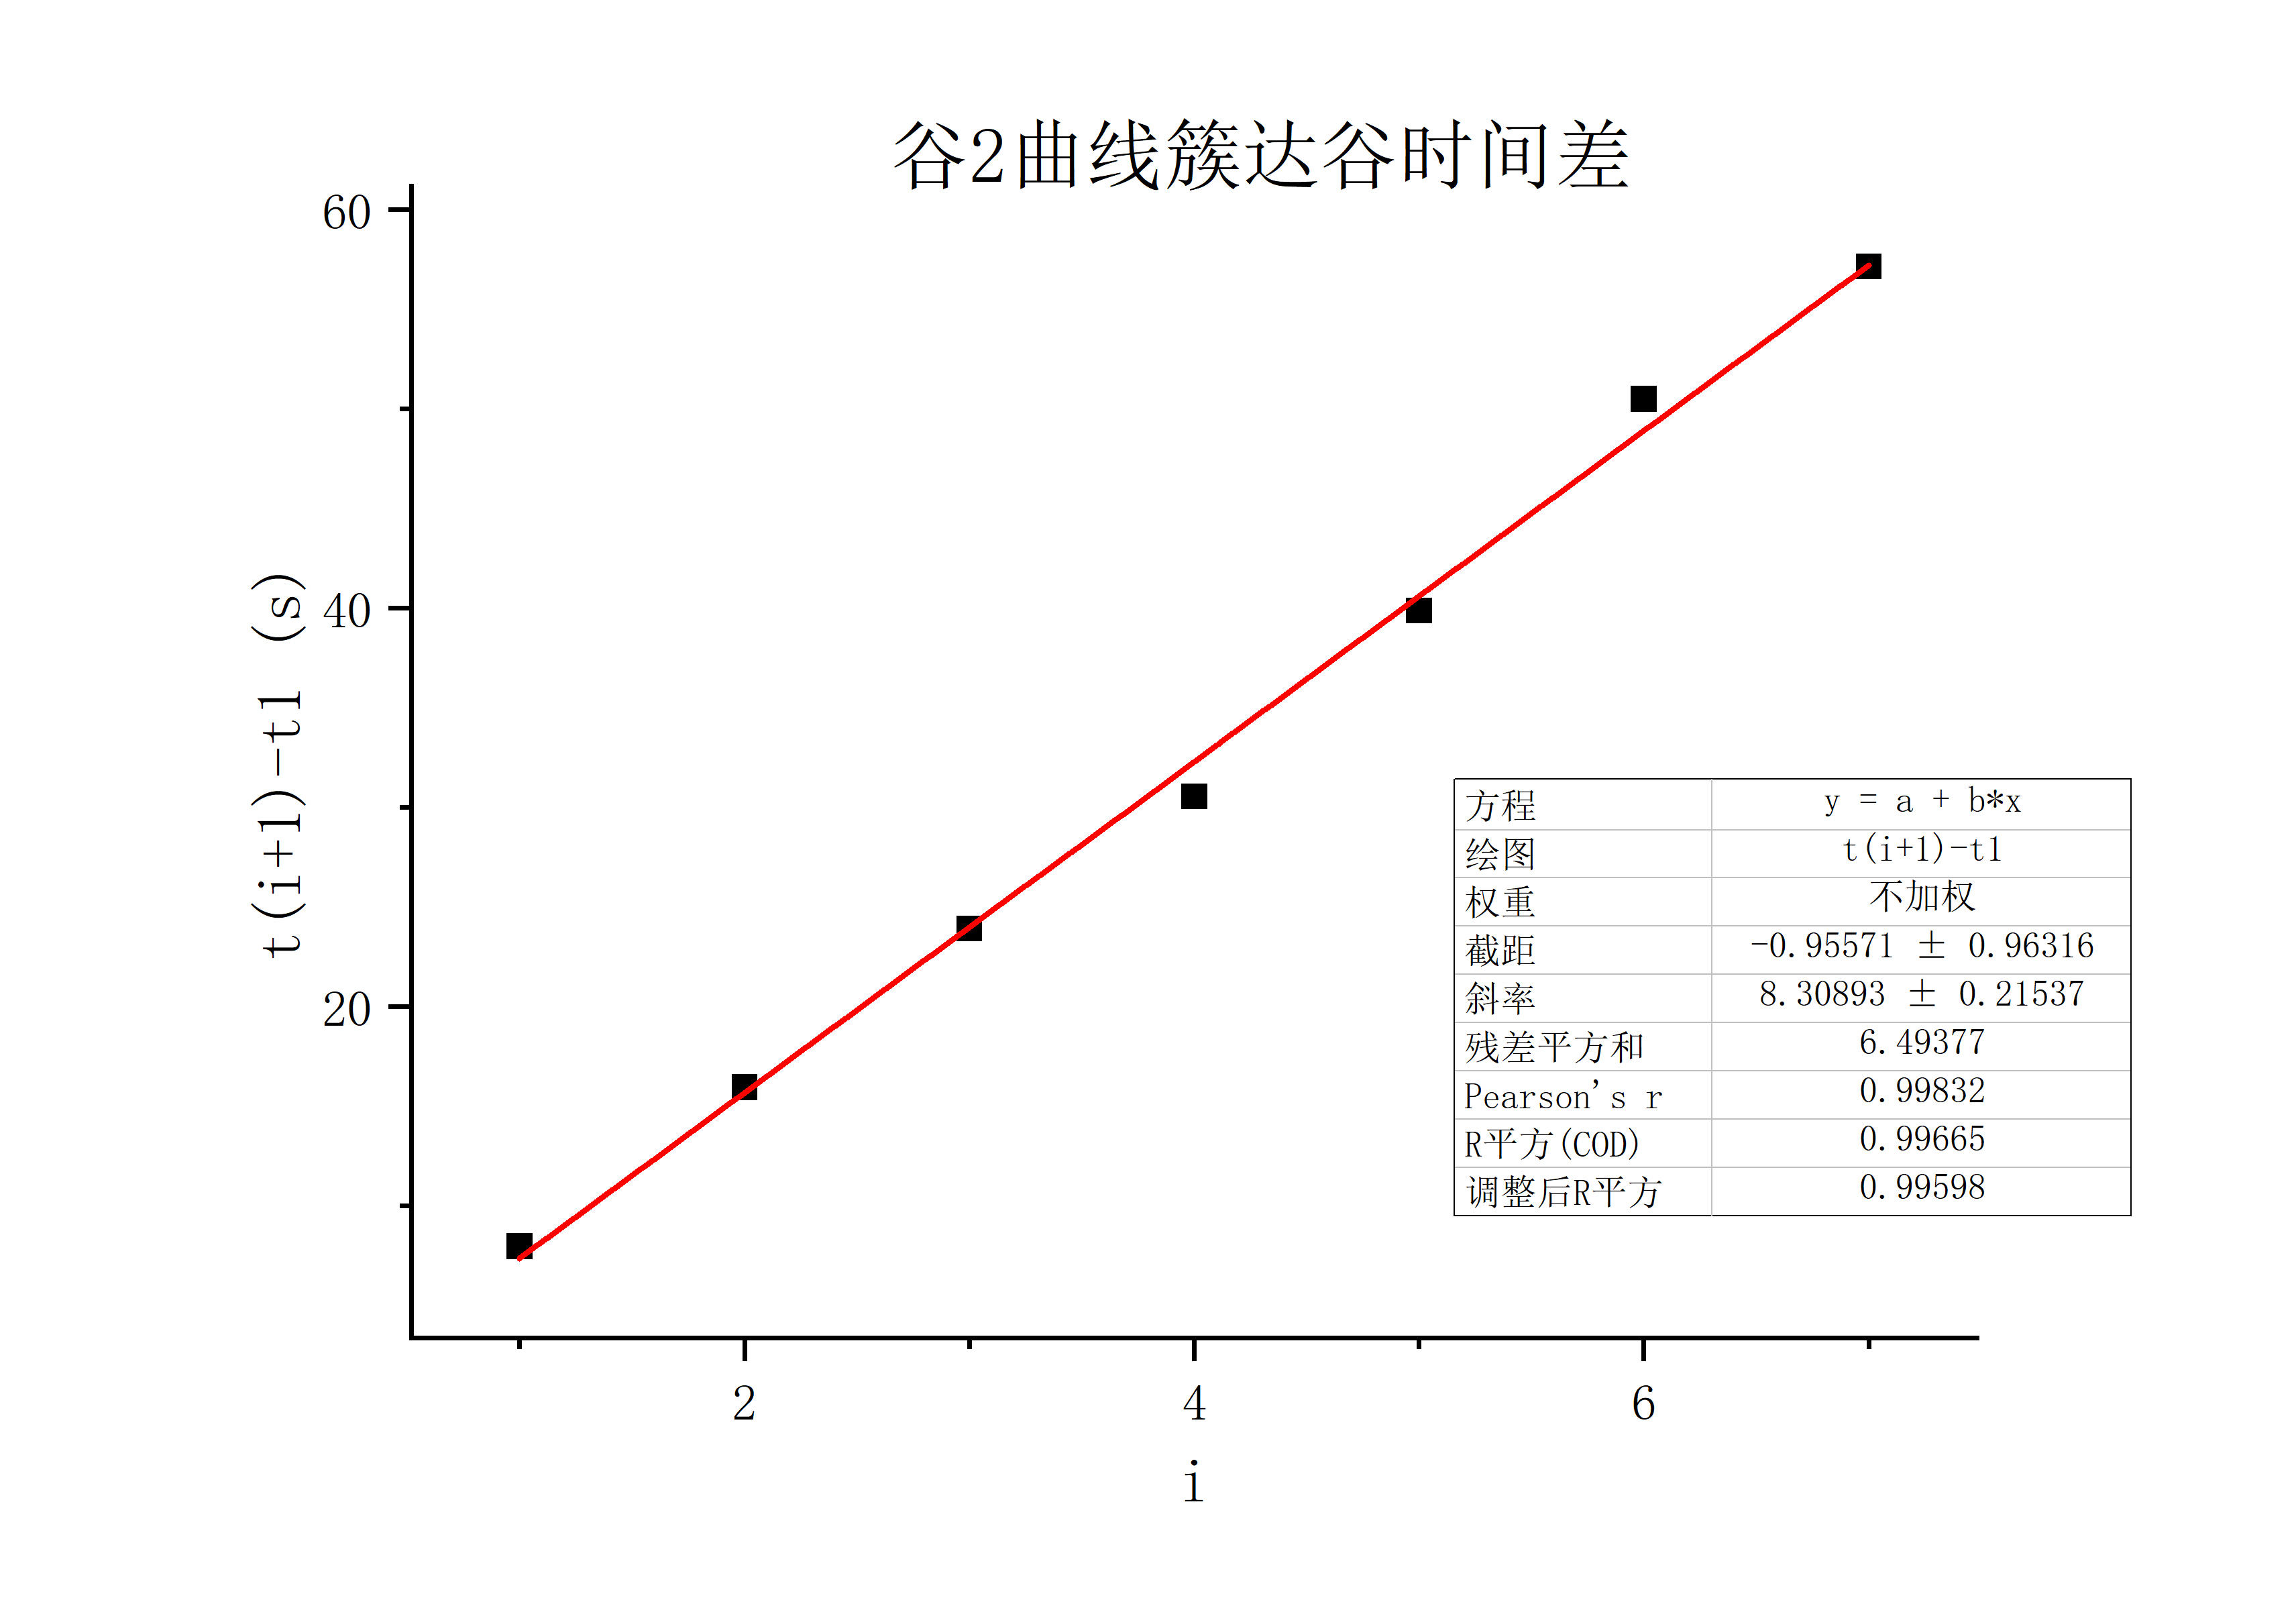
\includegraphics[width=0.7\textwidth]{谷2.jpg}
        \caption{谷2曲线簇达谷时间差}
    \end{figure*}

    曲线斜率$k=8.31s$,相关系数$r=0.999$。由此可计算得热波波速$v=\frac{l_0}{k}=2.41\times 10^{-3}m/s$。
    计算得到热导率
    $$\kappa=\frac{v^{2} c \rho}{4 \pi f}=\frac{v^{2} c \rho}{4 \pi} T_{\text {period }}=200W/m\cdot K$$

    用实验室提供的软件可以对曲线簇在峰值附近进行正弦函数拟合,然后根据拟合后的函数寻峰并利用最小二乘法计算热波波速,使用该软件利用峰曲线簇计算得到的波速为
    $$\kappa'=238.18W/m\cdot K$$

    \section{分析与讨论}
    \subsection{不同数据处理方法的比较}
    本次实验中用了2种方法对数据进行处理,一种是手动找出峰的位置和谷的位置,算出时间差用最小二乘法拟合,求出波速进而计算出热导率;
    另一种是利用软件再峰或者谷的位置附近用正弦函数对曲线进行拟合,再根据拟合后的正弦函数的峰或谷的位置计算出时间差求波速。
    从上面数据处理部分可以看出,前一种方法测得的热导率在$210W/m\cdot$左右,离铝热导率的参考值$238W/m\cdot$有大约$10\%$的误差;
    而后一种方法计算出的热导率,离参考值的误差还不到$3\%$。所以用正弦曲线进行拟合的方法有很高的优越性。

    这种现象一方面是因为原始曲线中,尤其是离热端比较近的位置的曲线,含有高次谐波的成分,因此不是完全的正弦曲线,峰和谷的位置会出现偏差;
    此外仪器记录数据毕竟是有时间差的,曲线放大之后可以看到是由一段一段的折线构成的,尤其是在峰和谷的位置,基本上都是一段平台,人眼判断峰和谷的位置也会出现误差。
    而正弦曲线拟合时,拟合的过程就可以规避掉高次谐波的影响,生成正弦曲线,而且拟合出来的正弦曲线峰和谷的位置唯一而且能直接由软件计算出,因此极大地提高了精确度。

    \subsection{误差来源的定性讨论}
    \begin{enumerate}
        \item [(1)] 系统误差 \\
        系统的传热不是理想的一维传热,虽然棒的长度远大于其直径、热电偶也是插在棒的中心轴线处、棒的四周包裹了绝热材料,但加热时并不完全是对轴线进行加热,因此不是理想的一维传热,会带来一定误差。

        由于加热的温度变化情况并不是完全的简谐规律,因此热波也不是理想的正弦波,而是有高次谐波的成分。虽然高次谐波衰减很快,但依然会使实验曲线的峰值和谷值位置发生变化,尤其是对比较靠近热端的几个位置,
        使得曲线的峰谷偏离正弦情况下的峰谷位置。

        热端冷却水流量调整得不是很合适,使得所测得的曲线不是完全对称。这会导致所测得的曲线偏离正弦曲线很远,峰谷的位置发生位移,造成误差。

        \item [(2)] 随机误差
        根据实验曲线寻找峰谷位置时,曲线放大后在极值处都会存在一个平台(因为机器是以一定时间频率测量温度的),所以曲线极值点的选取就是在平台上所对应的一段时间内选取一个点,这会使每个峰、谷对应的时间都产生随机误差。

        环境也会影响系统的传热。虽然装置的绝热做得比较好,但冷却水的波动却比较大,尤其是当其他组的仪器冷却水量有明显变化时,本组的水流量也会发生仪器可以检测到的变化。即使各组没有人调节水量,水管中的水流量本来就不是恒定的,
        也会引入随机误差。
    \end{enumerate}
\end{document}